\documentclass[Main.tex]{subfiles} 
\begin{document}

\section{Udviklingsv�rkt�jer}
%Kort beskrivelse af de anvendte udviklingsv�rkt�jer. 
%Herunder Scrumwise, SVN, Visual, Jenkins osv. Samt erfaringer der er gjort med disse.

Som n�vnt har den prim�re udviklingsprocess til dette projekt v�ret \textit{Scrum}.
\\
Under hele forl�bet er v�rkt�jet \textit{Scrum Wise}\footnote{http://www.scrumwise.com/ - for n�rmere indblik i Scrum Wise} blevet brugt til at h�ndtere projektback\-loggen og sprintbackloggen. V�rkt�jet er online-baseret, og det er meget nemt at g� til. Der er mulighed for at oprette, redigere, afslutte og s�tte statussen p� de forskellige opgaver, via det indbyggede taskboard. Derudover er der en burndown-chart, der g�r det nemt at overskue, hvordan det g�r med det aktuelle sprint.\\   
Dette v�rkt�j har gjort det nemt at benytte \textit{Scrum} som udviklingsprocess og virkelig givet den gennemskuelighed i projektetprocessen, hvilket er en af grundpillerne i \textit{Scrum}. Et lille eksempel p� \textit{Scrum Wise}, kan ses p� nedenst�ende billede(Ligger i stor st�rrelse i bilaget under Billeder/Scrum):
%\begin{figure}[H]
%\centering
%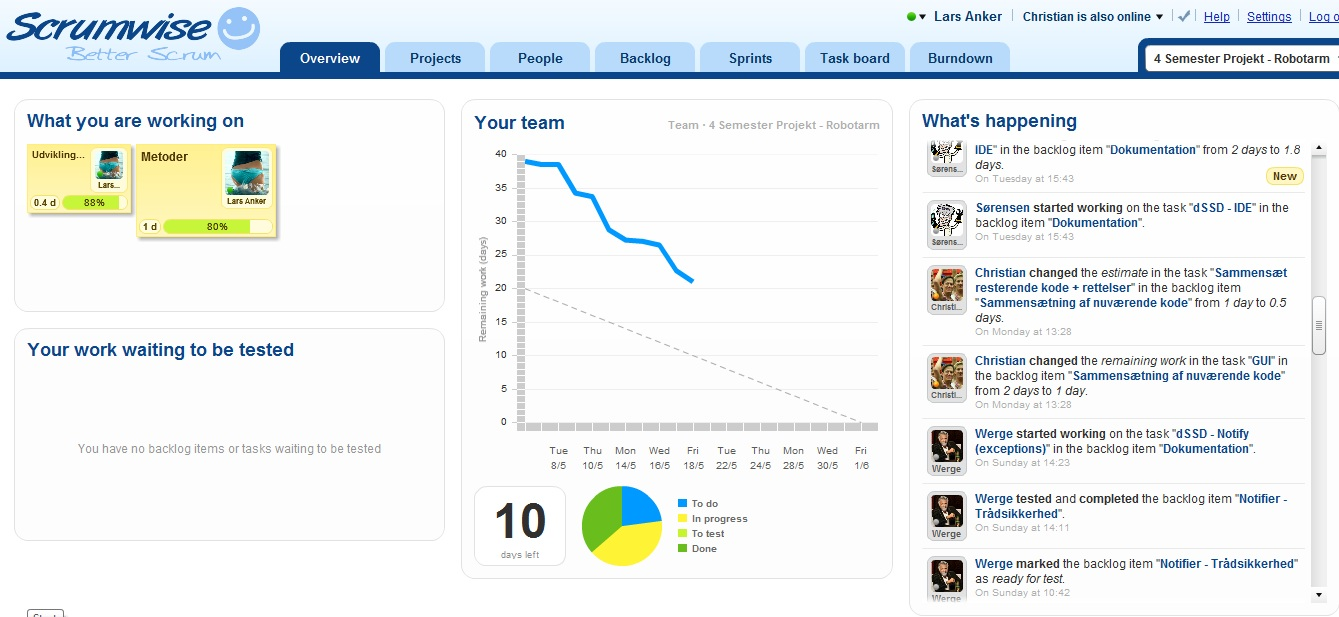
\includegraphics[scale=0.4]{Billeder/ScrumWise.jpg}
%\caption{Scrum Wise Overblik}
%\end{figure}
Til versionsstyring og revisionskontrol er der brugt \textit{SVN}. Programmerne \textit{SmartSVN} / \textit{TortoiseSVN} er benyttet til at styre den overordnede filh�ndtering. Derudover er \textit{Ankh\-SVN} ( et plugin til \textit{Microsoft Visual Studio}) blevet benyttet, hvilket sikrer en nem styring af solution-filer. Dette har givet en flydende versionsstyring uden store problemer. 
\\
Til test af koden er \textit{NUnit} blevet benyttet, sammen med frameworket \textit{Rhino Mocks}, der var en hj�lp til testskrivning. For at overskueligg�re hvor meget af koden der var testet, er \textit{DotCover} blevet brugt sammen med de ovenst�ende programmer.
\\
Derudover har hj�lpepluginet \textit{ReSharper} ligeledes hjulpet med syntax, opbygning af programmer og rettelser af navne p� attributter, variabler osv.
\\
\\
Alt tekstredigering er foreg�et i \textit{LaTeX}, hvilket har v�ret meget brugbart, da st�rre dokumenter kunne opdeles i forskellige filer, som kunne arbejdes p� individuelt.
Dette har tilladt, at flere gruppemedlemmer kunne redigere samme dokument uden der opstod konflikter. Desuden sikres, at de nyeste billeder og lignende altid er opdateret, da \textit{LaTeX} linker til disse i stedet for at inds�tte dem direkte ligesom i fx word.
\\
Brugen af \textit{LaTeX} har dog givet en del ekstra arbejde, da det var et nyt program for de fleste gruppemedlemmer. I sidste ende er den tabte tid dog blevet genvundet, da samlingen har fungeret smertefrit, og den grundl�ggende ops�tning ikke er blevet �delagt i takt med, at der er tilf�jet mere tekst.
\\
\\
Til brug til at lave diagrammer er programmet \textit{Visual Paradigm For UML}, samt \textit{Star UML} blevet benyttet. Disse programmer er fundet rigtig gode og nemme at arbejde med og dermed blevet de prim�re valg som diagramv�rkt�jer frem for for eksempel \textit{Microsoft Visio}.
\\
\textit{Microsoft Visio} er dog blevet benyttet, da det har v�ret glimrende til relationelle skemaer. Derudover er programmet \textit{DIA} blevet brugt til udformning af ER-diagrammer.

\end{document}
